% 繁星间漫步,陆巍的博客
\documentclass[UTF8]{ctexart}

% 注意宏包顺序,有可能会报错
\usepackage{geometry}% 用于页面设置
\usepackage{amssymb}% 数学符号
\usepackage{amsmath}% 数学相关支持
\usepackage{tikz}% 绘图
\usepackage{booktabs}% 增强表格功能
\usepackage{multirow}% 支持表格的多行合并
\usepackage{longtable}% 支持长表格跨页

\usetikzlibrary{shapes.gates.logic, circuits.logic.US, arrows.meta, positioning}

% 设置为A4纸
\geometry{
  a4paper,
  left = 19.1mm,
  right = 19.1mm,
  top = 25.4mm,
  bottom = 25.4mm
}

% tikz图形样式定义
% single arrow
\tikzset{
  Arrow1/.style = {
    draw,
    -{Latex[length = 2mm, width = 2mm]},
  }
}

% ------------------ 开始 -------------------
\begin{document}
\section{符号表}
\begin{longtable}{|p{9em}|p{15em}|p{15em}|}
  \bottomrule
  \hfil 主题 & \hfil 符号 & \hfil 意义\\
  \hline
  \multirow{15}{9em}{逻辑} & $\neg p$ & $p$的否定\\
  \cline{2-3}
    & $p\land q$ & $p$和$q$的合取\\
  \cline{2-3}
    & $p\lor q$ & $p$和$q$的析取\\
  \cline{2-3}
    & $p\oplus q$ & $p$和$q$的异或\\
  \cline{2-3}
    & $p\rightarrow q$ & $p$蕴含$q$\\
  \cline{2-3}
    & $p\leftrightarrow q$ & $p$和$q$的双条件\\
  \cline{2-3}
    & $p\equiv$ q & $p$和$q$的等价\\
  \cline{2-3}
    & $\mathbf{T}$ & 永真式\\
  \cline{2-3}
    & $\mathbf{F}$ & 矛盾式\\
  \cline{2-3}
    & $P(x_1, ... , x_n)$ & 命题函数\\
  \cline{2-3}
    & $\forall xP(x)$ & $P(x)$的全称量化\\
  \cline{2-3}
    & $\exists xP(x)$ & $P(x)$的存在量化\\
  \cline{2-3}
    & $\exists !xP(x)$ & $P(x)$的唯一存在量化\\
  \cline{2-3}
    & $\therefore$ & 所以\\
  \cline{2-3}
    & $p(S)q$ & $S$的部分正确性\\
  \hline
  \multirow{28}{9em}{集合} & $x\in S$ & $x$是$S$的成员\\
  \cline{2-3}
    & $x\notin S$ & $x$不是$S$的成员\\
  \cline{2-3}
    & $\{a_1, ... , a_n\}$ & 一个集合的元素列表\\
  \cline{2-3}
    & $\{x|P(x)\}$ & 集合构造器记法\\
  \cline{2-3}
    & $\mathbf{N}$ & 自然数集合\\
  \cline{2-3}
    & $\mathbf{Z}$ & 整数集合\\
  \cline{2-3}
    & $\rm\bf \mathbf{Z}^+$ & 正整数集合\\
  \cline{2-3}
    & $\mathbf{Q}$ & 有理数集合\\
  \cline{2-3}
    & $\mathbf{R}$ & 实数集合\\
  \cline{2-3}
    & $[a, b], (a, b)$ & 闭区间,开区间\\
  \cline{2-3}
    & $S=T$ & 集合等式\\
  \cline{2-3}
    & $\varnothing$ & 空集\\
  \cline{2-3}
    & $S\subseteq T$ & $S$是$T$的子集\\
  \cline{2-3}
    & $S\subset T$ & $S$是$T$的真子集\\
  \cline{2-3}
    & $|S|$ & $S$的基数\\
  \cline{2-3}
    & $\mathcal{P}(S)$ & $S$的幂集合\\
  \cline{2-3}
    & $(a_1, ... , a_n)$ & $n$元组\\
  \cline{2-3}
    & $(a, b)$ & 序偶\\
  \cline{2-3}
    & $A\times B$ & $A$和$B$的笛卡儿乘积\\
  \cline{2-3}
    & $A\cup B$ & $A$和$B$的并集\\
  \cline{2-3}
    & $A\cap B$ & $A$和$B$的交集\\
  \cline{2-3}
    & $A-B$ & $A$和$B$的差集\\
  \cline{2-3}
    & $\bar{A}$ & $A$的补集\\
  \cline{2-3}
    & $$\bigcup_{i=1}^nA_i$$ & $A_i$的并集,$i=1, 2, ... , n$\\
  \cline{2-3}
    & $$\bigcap_{i=1}^nA_i$$ & $A_i$的交集,$i=1, 2, ... , n$\\
  \cline{2-3}
    & $A\oplus B$ & $A$和$B$的对称差\\
  \cline{2-3}
    & $\aleph_0$ & 可数集的基数\\
  \cline{2-3}
    & $c$ & $\mathbf{R}$的基数\\
  \hline
  \multirow{22}{9em}{函数} & $f(a)$ & 函数$f$在$a$点的值\\
  \cline{2-3}
    & $f:A\leftrightarrow B$ & $f$是从$A$到$B$的函数\\
  \cline{2-3}
    & $f_1+f_2$ & 函数$f_1$和$f_2$的和\\
  \cline{2-3}
    & $f_1f_2$ & 函数$f_1$和$f_2$的积\\
  \cline{2-3}
    & $f(S)$ & 集合$S$在$f$之下的像\\
  \cline{2-3}
    & $_{\iota A}(_s)$ & $A$上的恒等函数\\
  \cline{2-3}
    & $f^{-1}(x)$ & $f$的逆\\
  \cline{2-3}
    & $f_\circ g$ & $f$和$g$的组合\\
  \cline{2-3}
    & $\lfloor x\rfloor$ & 下取整函数\\
  \cline{2-3}
    & $\lceil x\rceil$ & 上取整函数\\
  \cline{2-3}
    & $a_n$ & $\{a_i\}$中下标为$n$的项 \\
  \cline{2-3}
    & $$\sum_{i=1}^na_i$$ & $a_1, a_2, ... , a_n$之和\\
  \cline{2-3}
    & $$\sum_{\alpha\in S}\alpha_a$$ & $a_\alpha$之和,$\alpha\in S$\\
  \cline{2-3}
    & $$\prod_{i=1}^na_n$$ & $a_1, a_2, ... , a_n$之积\\
  \cline{2-3}
    & $f(x)是O(g(x))$ & $f(x)$是大$O_g(x)$ \\
  \cline{2-3}
    & $n!$ & $n$的阶乘\\
  \cline{2-3}
    & $f(x)$是$\Omega(g(x))$ & $f(x)$是大$\Omega(g(x))$\\
  \cline{2-3}
    & $f(x)$是$\Theta(g(x))$ & $f(x)$是大$\Theta(g(x))$\\
  \cline{2-3}
    & $\sim$ & 渐近于\\
  \cline{2-3}
    & $min(x, y)$ & $x$和$y$的最小值 \\
  \cline{2-3}
    & $max(x, y)$ & $x$和$y$的最大值 \\
  \cline{2-3}
    & $\approx$ & 约等于\\
  \hline
  \multirow{10}{9em}{整数} & $a\mid b$ & $a$整除$b$\\
  \cline{2-3}
    & $a\nmid b$ & $a$不整除$b$\\
  \cline{2-3}
    & $a\ \mathbf{div}\ b$ & $a$除以$b$所得的商\\
  \cline{2-3}
    & $a\ \mathbf{mod}\ b$ & $a$除以$b$所得的余数\\
  \cline{2-3}
    & $a\equiv b($mod $m)$ & $a$模$m$同余于$b$\\
  \cline{2-3}
    & $a\ne b($mod $m)$ & $a$模$m$不同余于$b$\\
  \cline{2-3}
    & $\mathbf{Z}_m$& 模$m$整数集\\
  \cline{2-3}
    & $(a_ka_{k-1}\cdots a_1a_0)_b$& 以$b$为基数的表示\\
  \cline{2-3}
    & gcd$(a, b)$& $a$和$b$的最大公因子\\
  \cline{2-3}
    & lcm$(a, b)$& $a$和$b$的最小公倍数\\
  \hline
  \multirow{9}{9em}{矩阵} & $[a_{ij}]$ & 矩阵,其中元素为$a_{ij}$\\
  \cline{2-3}
    & \textbf{\textit{A+B}}& 矩阵\textbf{\textit{A}}和\textbf{\textit{B}}的和\\
  \cline{2-3}
    & \textbf{\textit{AB}}& 矩阵\textbf{\textit{A}}和\textbf{\textit{B}}的积\\
  \cline{2-3}
    & \textbf{\textit{I}}$_n$& $n$阶单位矩阵\\
  \cline{2-3}
    & \textbf{\textit{A}}$^T$& \textbf{\textit{A}}的转置\\
  \cline{2-3}
    & \textbf{\textit{A}}$\vee$\textbf{\textit{B}}& 矩阵\textbf{\textit{A}}和\textbf{\textit{B}}的并\\
  \cline{2-3}
    & \textbf{\textit{A}}$\wedge$\textbf{\textit{B}}& 矩阵\textbf{\textit{A}}和\textbf{\textit{B}}的交\\
  \cline{2-3}
    & \textbf{\textit{A}}$\odot$\textbf{\textit{B}}& 矩阵\textbf{\textit{A}}和\textbf{\textit{B}}的布尔积\\
  \cline{2-3}
    & \textbf{\textit{A}}$^{[n]}$& \textbf{\textit{A}}的$n$次布尔幂\\
  \hline
  \multirow{12}{9em}{计数与概率} & $P(n, r)$ & $n$元素集合的$r$排列数\\
  \cline{2-3}
    & $C(n, r)$ & $n$元素集合的$r$组合数\\
  \cline{2-3}
    & $$\binom{n}{r}$$& $n$选$r$的二项式系数\\
  \cline{2-3}
    & $C(n;n_1,n_2,\cdots ,n_m)$& 多项式系数\\
  \cline{2-3}
    & $p(E)$& $E$的概率\\
  \cline{2-3}
    & $p(E|F)$& 给定$F$,$E$的条件概率\\
  \cline{2-3}
    & $E(X)$& 随机变量$X$的期望值\\
  \cline{2-3}
    & $V(X)$& 随机变量$X$的方差\\
  \cline{2-3}
    & $C_n$& 卡塔兰数\\
  \cline{2-3}
    & $N(P_{i_1}\cdots P_{i_n})$& 具有性质$P_{i_j}$的元素个数,$j=1,\cdots ,n$\\
  \cline{2-3}
    & $N(P^{'}_{i_1}\cdots P^{'}_{i_n})$& 不具有性质$P_{i_j}$的元素个数,$j=1,\cdots ,n$\\
  \cline{2-3}
    & $D_n$& $n$个元素的错排数\\
  \hline
  \multirow{4}{9em}{关系} & $S\circ R$ & 关系$S$和$R$的复合\\
  \cline{2-3}
    & $R^n$& 关系$R$的$n$次幂\\
  \cline{2-3}
    & $R^{-1}$& 逆关系\\
  \cline{2-3}
    & $s_C$& 条件$C$的选择操作\\
  \cline{2-3}
    & $Pi_1,i_2,\cdots i_m$& 投影\\
  \cline{2-3}
    & $J_p(R, S)$& 联合\\
  \cline{2-3}
    & $\Delta$& 对角线关系\\
  \cline{2-3}
    & $R^*$& $R$的连通性关系\\
  \cline{2-3}
    & $a\sim b$& $a$等价于$b$\\
  \cline{2-3}
    & $[a]_R$& $a$的$R$等价类\\
  \cline{2-3}
    & $[a]_m$& 模$m$的同余类\\
  \cline{2-3}
    & $(S, R)$& 由集合$S$和偏序$R$构成的偏序集\\
  \cline{2-3}
    & $a\prec b$& $a、b$有$\prec$关系\\
  \cline{2-3}
    & $a\succ b$& $a、b$有$\succ$关系\\
  \cline{2-3}
    & $a\preccurlyeq b$& $a、b$有$\preccurlyeq$关系\\
  \cline{2-3}
    & $a\succcurlyeq b$& $a、b$有$\succcurlyeq$关系\\
  \hline
  \multirow{26}{9em}{图和树} & $(u, v)$ & 有向边\\
  \cline{2-3}
    & $G=(V, E)$& 以$V$为点集、$E$为边集的图\\
  \cline{2-3}
    & $\{u, v\}$& 无向边\\
  \cline{2-3}
    & $deg(v)$& 顶点$v$的度数\\
  \cline{2-3}
    & $deg^-(v)$& 顶点$v$的入度\\
  \cline{2-3}
    & $deg^+(v)$& 顶点$v$的出度\\
  \cline{2-3}
    & $K_n$& $n$个顶点的完全图\\
  \cline{2-3}
    & $C_n$& 大小为$n$的圈图\\
  \cline{2-3}
    & $W_n$& 大小为$n$的轮图\\
  \cline{2-3}
    & $Q_n$& $n$立方体图\\
  \cline{2-3}
    & $K_{n,m}$& 大小为$n、m$的完全二分图\\
  \cline{2-3}
    & $G-e$& $G$删除边$e$后的子图\\
  \cline{2-3}
    & $G+e$& $G$增加边$e$所得的图\\
  \cline{2-3}
    & $G_1\cup G_2$& $G_1$和$G_2$的并\\
  \cline{2-3}
    & $a,x_1,\cdots ,x_{n-1},b$& 从$a$到$b$的通路\\
  \cline{2-3}
    & $a,x_1,\cdots ,x_{n-1},a$& 回路\\
  \cline{2-3}
    & $\kappa (G)$& $G$的顶点连通度\\
  \cline{2-3}
    & $\lambda (G)$& $G$的边连通度\\
  \cline{2-3}
    & $r$& 平面图的面数\\
  \cline{2-3}
    & deg($R$)& 面$R$的度数\\
  \cline{2-3}
    & $\chi (G)$& $G$的着色数\\
  \cline{2-3}
    & $m$& 根树中内点的最大子树数\\
  \cline{2-3}
    & $n$& 根树中的顶点数\\
  \cline{2-3}
    & $i$& 根树中的内点数\\
  \cline{2-3}
    & $l$& 根树中的叶子数\\
  \cline{2-3}
    & $h$& 根树的高度\\
  \hline
  \multirow{10}{9em}{布尔代数} & $\bar{x}$ & 布尔变量$x$的补\\
  \cline{2-3}
    & $x+y$& $x$和$y$的布尔和\\
  \cline{2-3}
    & $x\cdot y$(或$xy$)& $x$和$y$的布尔积\\
  \cline{2-3}
    & $B$& \{(0,1)\}\\
  \cline{2-3}
    & $F^d$& $F$的对偶\\
  \cline{2-3}
    & $x|y$& $x$ NAND $y$\\
  \cline{2-3}
    & $x\downarrow y$& $x$ NOR $y$\\
  \cline{2-3}
    & 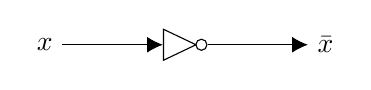
\begin{tikzpicture}
      \draw
        (0,0)node[not gate US, draw, logic gate inputs=out](not1){}
        ([xshift=-15mm]not1.input)node(x1){$x$}
        ([xshift=15mm]not1.output)node(x2){$\bar{x}$}
        (x1)[Arrow1] -- (not1.input);
      \draw([xshift=1.5mm]not1.east)[Arrow1] -- (x2);
    \end{tikzpicture}
    & 非门\\
  \cline{2-3}
    & 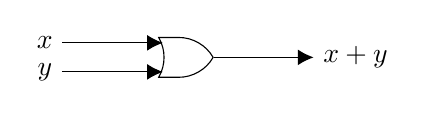
\begin{tikzpicture}
      \draw
        (0,0)node[or gate US, draw](or1){}
        ([xshift=-15mm, yshift=1mm]or1.input 1)node(x1){$x$}
        ([xshift=-15mm, yshift=-1mm]or1.input 2)node(y1){$y$}
        ([xshift=18mm]or1.output)node(x2){$x+y$}
        (x1)[Arrow1] -- ([yshift=1mm]or1.input 1);
      \draw (y1)[Arrow1] -- ([yshift=-1mm]or1.input 2);
      \draw (or1.output)[Arrow1] -- (x2);
    \end{tikzpicture}
    & 或门\\
  \cline{2-3}
    & \begin{tikzpicture}
      \draw
        (0,0)node[and gate US, draw](and1){}
        ([xshift=-15mm, yshift=1mm]and1.input 1)node(x1){$x$}
        ([xshift=-15mm, yshift=-1mm]and1.input 2)node(y1){$y$}
        ([xshift=15mm]or1.output)node(x2){$xy$}
        (x1)[Arrow1] -- ([yshift=1mm]and1.input 1);
      \draw (y1)[Arrow1] -- ([yshift=-1mm]and1.input 2);
      \draw (and1.output)[Arrow1] -- (x2);
    \end{tikzpicture}
    & 与门\\
    \hline
    \multirow{16}{9em}{语言和有限状态机} & $\lambda$ & 空串\\
    \cline{2-3}
      & $xy$& $x$和$y$的连接\\
    \cline{2-3}
      & $l(x)$& 串$x$的长度\\
    \cline{2-3}
      & $w^R$& $w$的反串\\
    \cline{2-3}
      & $(V,T,S,P)$& 短语结构文法\\
    \cline{2-3}
      & $S$& 开始符号\\
    \cline{2-3}
      & $w\rightarrow w_1$& 产生式\\
    \cline{2-3}
      & $w_1\Rightarrow w_2$& $w_2$可由$w_1$直接派生\\
    \cline{2-3}
      & $w_1\stackrel{*}{\Rightarrow}w_2$& $w_2$可由$w_1$派生\\
    \cline{2-3}
      & $<A>::=<B>c|d$& 巴克斯-诺尔范式\\
    \cline{2-3}
      & $(S,I,O,f,g,s_0)$& 带输出的有限状态机\\
    \cline{2-3}
      & $s_0$& 开始状态\\
    \cline{2-3}
      & $AB$& 集合$A$和$B$的连接\\
    \cline{2-3}
      & $A^*$& $A$的Kleene闭包\\
    \cline{2-3}
      & $(S,I,f,s_0,F)$& 不带输出的有限状态自动机\\
    \cline{2-3}
      & $(S,I,f,s_0)$& 图灵机\\
  \toprule
\end{longtable}
\end{document}
